\chapter{绪论:初识机器学习}

\begin{center}
学而不思则罔,思而不学则怠!
\end{center}

\begin{flushright}
---孔子    
\end{flushright}

\section{欢迎参加机器学习课程}
机器学习是最激动人心的技术。在很多方面都使用了机器学习技术。机器学习主要的应用方向:
\begin{itemize}
\itemsep=3pt
\parskip=0pt
\item 数据挖掘
\item 在无法手动编写的程序中的应用
\item 在私人定制程序中的应用
\end{itemize} 

\section{什么是机器学习}

本节课程的主要内容有两个:
\begin{enumerate}[1)]
\item 机器学习的定义
\begin{newdef}[Arthur Samuel]
\large 在没有明确设置的情况下使计算机具有学习能力的研究领域。
\end{newdef}

\begin{newdef}[Tom Mitchell]
\large 对于某类任务T和性能度量P,如果一个计算机程序在T上以P衡量的
性能随着经验E而自我完善,那么我们称这个计算机程序在从经验E学习。\cite{MachineLearning}
\end{newdef}
\item 在什么情况下使用机器学习

常用机器学习算法一般可以分为两类:
\begin{itemize}
\item 监督学习{\color{red} ---教会计算机做某件事情。}
\item 无监督学习{\color{red} ---让计算机自己学习。}
\end{itemize}

\end{enumerate}

\section{监督学习}

\subsection{回归问题}
使用波特兰房屋价格的例子来说明监督学习,采集的数据如下图1.1所示,横轴表示的是平方英尺数,纵轴是不同房子的价格,单位是千美元。

\begin{figure}[!hbtp]
\centering
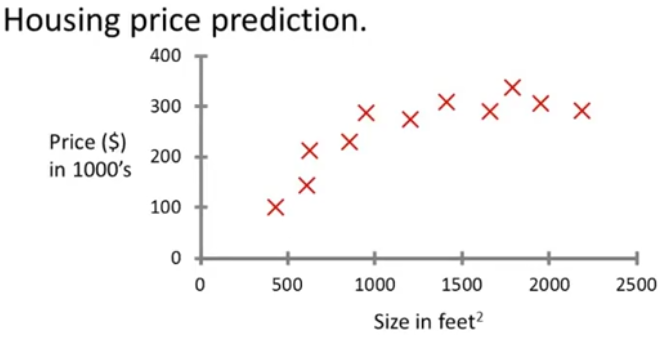
\includegraphics[width=0.8\textwidth]{room_price.png}
\caption{Room Price\label{figur:root_price}}
\end{figure}

假设你的朋友有一栋750平方英尺的房子,他想要卖掉房子,需要预测一下能够卖多少钱,此时学习算法能够有什么帮助呢?
根据数据画一条直线,或者说一条直线拟合数据,如图1.2所示,由此看房子大约可以卖15万美元。
\begin{figure}[H]
\centering
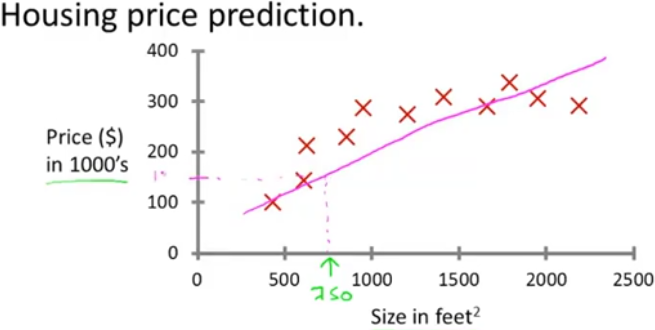
\includegraphics[width=0.8\textwidth]{room_price_1.png}
\caption{Room Price fitting straight\label{figur:root_price_1}}
\end{figure}

当然这并不是唯一能使用的学习算法,例如除了使用一条直线来拟合之外,还可以采用二阶函数或者二阶多项式来拟合,这样可能会更好,如图1.3
所示,此时你再做预测,看上去房子可以卖出接近20万美元。
\begin{figure}[!hbtp]
\centering
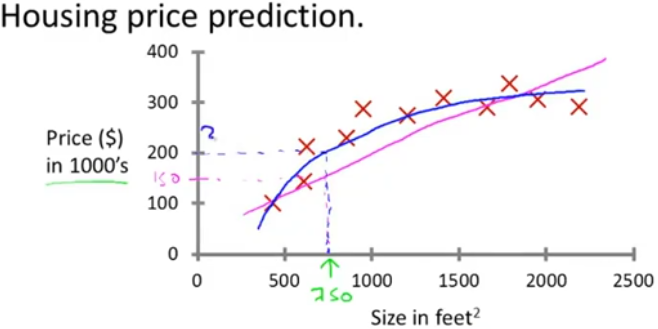
\includegraphics[width=0.8\textwidth]{room_price_2.png}
\caption{Room Price Second Derivative\label{figur:root_price_2}}
\end{figure}

而我们需要讨论的一件事就是如何选择如何决定,是采用直线来拟合数据,还是采用二阶函数来拟合,
当然无论采用哪个模型都不会让你的朋友房子的价格卖的更好,但这是一个学习算法很好的例子,这
是一个监督学习算法的例子。

监督学习是指我们给算法一个数据集,其中包含了正确答案,也就是说我们给他一个房价数据集,在
这个数据集中的每个样本,我们都给出正确的价格,即这个房子实际卖价,算法的目的就是给出更多
的正确答案,例如为你朋友想要卖掉的这所新房子给出估价,用更专业的术语来说,它也被称为回归问题。
这里的回归问题指的是我们想要预测连续的数值输出,也就是价格,技术上而言价格能够被圆整到分,
因此是一个离散值,但通常我们认为房价是一个实数标量或是连续值,回归问题是我们设法预测连续值
的属性。

\subsection{分类问题}


\section{无监督学习}
无监督学习告诉你更多哦。
\section{问题}
学习之后就要思考问题。